\subsection{Bedienung}
Die Software zur Bedienung wurde in drei Teile gestaltet. Hardwaremäßig wurde nur das geringste an Elementen verwendet. Die drei Bedienelemente sind jeweils Aktiv High am Mikrocontroller geschaltet mittels einem Taster-Pull-Up-Schaltkreis \ref{fig:SwitchPullUp_Software}. Der Pull-Up Widerstand ist $10k\Omega$, der mit einem Taster auf Erde verbunden wird.

\begin{figure}[h]
	\centering
		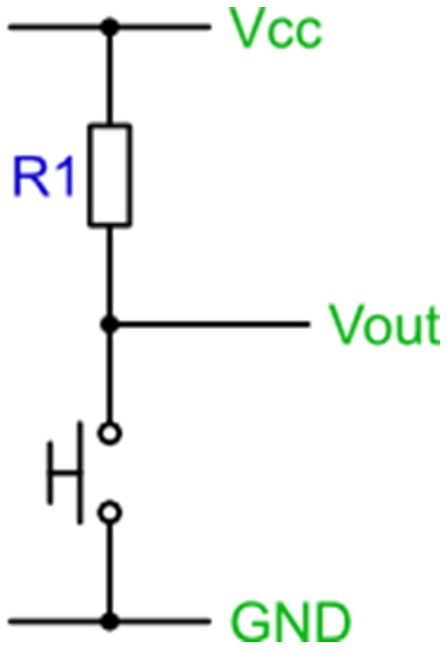
\includegraphics[width=0.25\textwidth]{switchpullupcircuit.jpg}
	\caption{Taster-Pull-Up-Schaltkreis}
	\label{fig:SwitchPullUp_Software}
\end{figure}


%ISR (TIMER0_OVF_vect)
Der Timer-Interrupt im Mikrocontroller ruft alle 16ms eine Funktion auf, die den Taster entprellt, aber auch die Länge des Tasterzustandes registriert.
%button |= ~old_button & current_button & BUTTONMASK;
Der Taster (button) wird als gedrückt erkannt, wenn die Inverse vom alten Zustand (old\_button), dem momentanen Zustand (current\_button) und der Pinmaske (BUTTONMASK) übereinstimmen.
%if (button)
Mit mehreren If-Bedingungen werden das Auf- und Abwärtszählen, das automatische Zählen und der Modus gewählt. Wird zum Beispiel der Aufwärtszähler kurz gedrückt, setzt das Programm die Verzögerung des automatischen Zählers (autorepeat) präventiv auf 50, das ungefähr zwei Sekunden entspricht. Nachfolgend wird der Wert um Eins dekrementiert. Eine integrierte If-Bedingung begrenzt den Aufwärtszähler bei 100 und setzt den Wert auf 20 zurück.
\newline
Der gleiche Verlauf wurde programmiert zum Abwärtszählen mit kurzem drücken.
\newline
Als nächstes wurde das automatische Zählen programmiert. Auf die If-Bedingung wird eingegangen, wenn der momentan gedrückte Taster (current\_button) und die Tastermaske (BUTTONUP) Eins ergeben. Folglich wird der automatische Zähler ab dem gesetzten Wert, in dem Fall ab 50, dekrementiert bis der Wert Null erreicht hat, dann wird \textit{autorepeat} nochmals auf 50 gesetzt für eine allfällige Fortsetzung des automatischen Zählens.
\newline
Bevor die eigentliche Rechnung erfolgt wird der Taster (button) gleich der Tastermaske (z.B. BUTTONUP) gesetzt. Die Rechnung ist einfach zu realisieren, denn ein Integer ist bekanntlich eine ganze Zahl. Wird zuerst die Bestrahlungsstärke durch Zehn dividiert und umgekehrt mit Zehn multipliziert verliert die Zahl die Ziffer nach dem Koma und eine ganze Zehnerzahl entsteht. Dieser wird nun Zehn hinzugefügt oder abgezogen.
\newline
Für das automatische verringern der Bestrahlungsstärke wurde eine weitere Variable erschaffen. Die Differenz zwischen dem momentanen Wert und der errechneten Zehnerzahl nach der obigen Rechnung wird in die neue Variable gespeichert. Ist die Differenz Zehn wird die obige Rechnungsmethode verwendet, ist jedoch die Differenz grösser als Zehn wird bei der Rechnungsmethode auf das verringern um Zehn verzichtet. Das hat zur Sache, dass wenn z.B. die Zahl 55 automatisch verringert wird nicht gleich auf 40 gesprungen wird, statt auf 50. Zuletzt wird bei beiden Automatismen die Prüfung der Grenzwerte angewendet, damit die Bestrahlungsstärke im Bereich bleibt.
\newline
Für den Modus wurde ein Array der Länge drei initialisiert und mit den Texten: \textit{NORMAL}, \textit{VERSCHMUTZT}, \textit{TEILDEFEKT}, gefüllt. Wird der Taster (MODE) gedrückt inkrementiert eine Laufvariable und gibt den entsprechenden Text des Arrays auf dem Display aus.